% !TeX encoding = UTF-8
% !TeX spellcheck = it_IT
% !TeX root = MatDiz.tex
\chapter{P}
\vspace{5mm}
\lemma{Papiro di Rhind}\pointsto~\seeentry{Rhind Henry} 
noto anche come papiro di Ahmes\pointsto~\seeentry{Ahmes}\index{Ahmes} uno scriba che lo  compilò nel 1650 a.C partendo da una fonte di tre secoli prima. Fu trovato a Luxor da Henry Rhind\index{Rhind Henry} che nel 1858 lo donò al 
\foreignlanguage{english}{British Museum}. Il papiro inizia con un elenco di frazioni nella forma $2/n$ che sono espresse come somma di frazioni egizie. Il papiro  contiene una raccolta di ottantasette  problemi. Viene considerato come una delle maggiori fonti della matematica egizia. \cite{Gheverghese2000}
\begin{figure}[!htb]
\def\FrameCommand{\fboxsep=\FrameSep \colorbox{shadecolor}}% da def\FrameCommand{\fboxsep=\FrameSep\colorbox{shadecolor}}% da "shaded"
\begin{MakeFramed}{\advance\hsize-\width \FrameRestore}%    da "framed"
\begin{center}%
\textcolor{StrongGray}{\textsf{Moltiplicazione egizia}}%
\par%
\vspace*{-\smallskipamount}%
\vrule height 0.8pt width 56mm%
\end{center}%
\begin{small}%
La moltiplicazione egizia si basa sulla duplicazione. Supponiamo che il nostro scriba volesse moltiplicare settanta per venticinque. Per prima  cosa doveva decidere chi stava per essere essere moltiplicato. 

Poniamo che venticinque moltiplichi settanta. Ahmes\index{Ahmes} avrebbe organizzato il lavoro in questo modo. Nella prima riga scriveva uno e settanta. La tabella è costruita in modo che ogni riga è il doppio della riga precedente. Questo procedimento di duplicazione termina quando il numero a sinistra supera, in questo caso, venticinque.%
\begin{center}
\begin{tabular}{LL}
\toprule 
1 & 70 \\ 
2 & 140 \\ 
4 & 280 \\ 
8 & 560 \\ 
16 & 1120 \\ 
\bottomrule
\end{tabular} 
\end{center}
Per prima cosa il nostro scriba avrebbe individua to nella colonna di sinistra i numeri la cui somma è uguale a 25 \[ 25=1+8+16\] Successivamente avrebbe sommato i corrispondenti numeri della seconda colonna ottenendo il prodotto. In notazione moderna\[ 70\times 25=70+560+1120=1750 \]Il procedimento si basa sul fatto che ogni numero può essere scritto come somma di potenze del  due \[25=1\cdot 2^0+0\cdot 2^2+1\cdot 2^3+1\cdot2^4  \] e successivamente l'uso della proprietà distributiva.
\end{small}%
\vspace*{-\smallskipamount}%
\end{MakeFramed}%
\end{figure}%
\lemma{parabola}Luogo geometrico dei punti del piano equidistanti da un punto fisso detto fuoco e da una retta fissa detta direttrice.
\lemma{parallele} Si dice di rette o piani che non hanno punti in comune. \llemma{p. postulato} Il quinto postulato\pointsto~\seeentry{postulato}  di Euclide\pointsto~\seeentry{Euclide} recita  \textit{Data una retta e un punto esterno ad esso per il punto passa una e una sola retta parallela alla retta data.}. 
\lemma{parallelepipedo} Poliedro a sei facce due a due parallele.
\lemma{parallelogramma} Quadrilatero con i lati opposti sono paralleli e uguali.
\lemma{parentesi} in un'espressione variano l'ordine con cui devono essere svolte delle operazioni. Vennero introdotte da {Viète\pointsto~\seeentry[Viete Francois]{Viète François} nel 1593 circa\cite{Kline1972}\index{Viète Fraçois}
\lemma{pari} Un numero è pari se è un multiplo\pointsto~\seeentry{multiplo} del due.
\lemma{Pascal Blaise} (1623-1662)\index{Pascal Blaise}
\begin{figure}
	\centering\scaptionb{Blaise Pascal (1623-1662)}
	\label{fig:pascalblaise}
	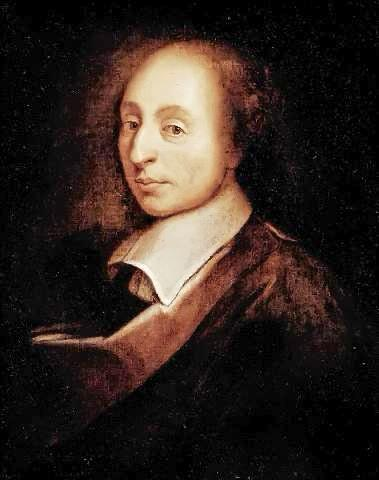
\includegraphics[width=0.7\linewidth]{Figure/P/Pascal_Blaise}
\end{figure}Ragazzo prodigio diede molti contributi alla matematica finché, dopo un esaurimento nervoso, di diede alla teologia. Fondamentali i suoi contributi al calcolo della probabilità. Introdusse il concetto di pressione. Nel 1642 costruì la sua prima macchina calcolatrice, la pascalina.
\lemma{Peano Giuseppe}  (1858-1932)\index{Peano Giuseppe}
\lemma{perimetro}Misura della lunghezza del contorno di una figura piana\pointsto~\seeentry{f. piana}. Viene indicato  con il simbolo $2P$.%
\lemma{permutazione}Dati n elementi distinti, tutti i possibili raggruppamenti formati da n oggetti, senza ripetizioni,  e che differiscano solo per l'ordine con cui sono formati si chiamano permutazioni semplici. Il simbolo è $P_n$, dove n indica il numero degli elementi. Il numero delle permutazioni è  $P_n=n!$.
\lemma{perpendicolare} Una retta è perpendicolare ad un'altra retta se ha un solo punto in comune con essa e forma quattro angoli retti.
\lemma{piano}Per Euclide\pointsto~\seeentry{Euclide}\index{Euclide} ente geometrico fondamentale insieme a punto e retta. \llemma{p. cartesiano}%
\begin{figure}[!htb]
	\def\FrameCommand{\fboxsep=\FrameSep \colorbox{shadecolor}}% da def\FrameCommand{\fboxsep=\FrameSep\colorbox{shadecolor}}% da "shaded"
	\begin{MakeFramed}{\advance\hsize-\width \FrameRestore}%    da "framed"
		\begin{center}%
\textcolor{StrongGray}{\textsf{Divisione egizia}}%
			\par%
			\vspace*{-\smallskipamount}%
			\vrule height 0.8pt width 56mm%
		\end{center}%
		\begin{small}%
		La divisione segue uno schema simile alla moltiplicazione. Poniamo di voler trovare il risultato di \[ 750\div 15\]
		\begin{center}
			\begin{tabular}{cc}
			\toprule
				1 & 15 \\ 
				2 & 30 \\ 
				4 & 60 \\ 
				8 & 120 \\ 
				16 & 240 \\ 
				32 & 480 \\ 
			\bottomrule
			\end{tabular} 
		\end{center}
	Nella colonna di destra individuo i numeri la cui somma è il dividendo\[750=480+240+30\] La somma dei corrispondenti numeri della colonna di sinistra da il quoziente\[ 50=2+16+32\]
		\end{small}%
		\vspace*{-\smallskipamount}%
	\end{MakeFramed}%
\end{figure}%
\lemma{Peirce Benjamin}(1809-1880)\index{Peirce Benjamin}
\lemma{pi greco}Numero irrazionale\pointsto~\seeentry{n. irrazionale} trascendente\pointsto~\seeentry{n. trascendente} corrispondente al rapporto tra una circonferenza\pointsto~\seeentry{circonferenza} e il suo  diametro\pointsto~\seeentry{diametro}. Il simbolo $\pi$ fu introdotto nel 1706 da  William Jones\pointsto~\seeentry{Jones William}.
%
%\begin{figure}[!htb]
%	\def\FrameCommand{\fboxsep=\FrameSep \colorbox{shadecolor}}% da def\FrameCommand{\fboxsep=\FrameSep\colorbox{shadecolor}}% da "shaded"
%	\begin{MakeFramed}{\advance\hsize-\width \FrameRestore}%    da "framed"
%		\begin{center}%
%			\textcolor{StrongGray}{\textsf{Pi greco}}%
%			\par%
%			\vspace*{-\smallskipamount}%
%			\vrule height 0.8pt width 56mm%
%		\end{center}%
%		\begin{small}%
%			Durante i secoli vi sono state varie rappresentazioni numeriche di $\pi$ 
%		\begin{center}
%			\begin{tabularx}{\linewidth}{XlX}
%	
%				1650 a.C. & Papiro di  Ahmes & $\pi\approx 3.16$\\ 
%			1600 a.C. & Tavoletta di Susa & $\pi\approx 3.125$\\ 
%			800 -- 500 a.C.	&Sulbasutra  &  $\pi\approx 3.09$\\ 
%			250 a.C. 	&Archimede  &   $\pi\approx\num{3.14}$\\ 
%			150 a.C. 	&Umasvati &   $\pi\approx\num{3.16}$\\ 
%			260 d.C. 	&Liu Hui  &   $\pi\approx\num{3.1416}$\\ 
%		480 d.C. 	&Tsu Chhung-Chih  &  $\num{3.1415926}<\pi<\num{3.1415927}$\\
%			500 d.C.	&Arybhata  & $\pi\approx\num{3.1416}$ \\ 
%			1400	&Madhava  & $\pi~\approx~\num{3.14159265359} $\\ 
%				&  &  \\ 
%				&  &  \\ 
%			\bottomrule
%			\end{tabularx} 
%		\end{center}
%		\end{small}%
%		\vspace*{-\smallskipamount}%
%	\end{MakeFramed}%
%\end{figure}%
\lemma{piramide} Poliedro costituito da una base poligonale e da altre formate da triangoli con il vertice in comune.
\lemma{Pitagora}\index{Pitagora}\llemma{P. teorema} In un triangolo rettangolo la somma dei quadrati costruiti su i cateti è equivalente al quadrato costruito sull'ipotenusa
\lemma{poliedro}figura solida delimitata da poligoni non complanari piani. Ogni lato è in comune a due di essi. Il punto di incontro di più lati è chiamato vertice.
\lemma{poligonale}Insieme ordinato di segmenti consecutivi non adiacenti.\llemma{p. aperta} Una poligonale è aperta se il primo estremo e l'ultimo non si intersecano. Una poligonale è aperta intrecciata se il primo estremo e l'ultimo non si intersecano ma i segmenti hanno almeno  un punto in comune.\llemma{p. chiusa} Una poligonale è chiusa se il primo estremo e l'ultimo estremo  si intersecano. Una poligonale è chiusa intrecciata se il primo estremo e l'ultimo  si intersecano e i segmenti hanno almeno  un punto in comune.
\lemma{poligono}Figura geometrica piana\pointsto~\seeentry{f. piana} limitata da tre o più segmenti\pointsto~\seeentry{segmento} che formino una poligonale chiusa non intrecciata\pointsto~\seeentry{p. chiusa}.
\lemma{polinomio}Somma di monomi non simili.
\lemma{postulato}
\lemma{prodotto} 
\lemma{punto}Per Euclide\pointsto~\seeentry{Euclide}\index{Euclide} ente geometrico fondamentale insieme a piano e retta.\llemma{p. medio}Punto equidistante dagli estremi di un segmento\pointsto~\vedilemma{segmento}.
\begin{table}[t]
\scaptionb{Tabella delle frazioni 2/n del papiro Rhind}\label{PapiroRhindtabella}%
\centering%
\begin{shadedtabular}[paglierino]{LL}
\toprule	
\frac{2}{3}=\frac{1}{2}+\frac{1}{6}&\frac{2}{5}=\frac{1}{3}+\frac{1}{15}\\
\frac{2}{7}=\frac{1}{4}+\frac{1}{28}&\frac{2}{9}=\frac{1}{6}+\frac{1}{18}\\
\frac{2}{11}=\frac{1}{6}+\frac{1}{66}&\frac{2}{13}=\frac{1}{8}+\frac{1}{52}+\frac{1}{104}\\

\frac{2}{15}=\frac{1}{10}+\frac{1}{30}&\frac{2}{17}=\frac{1}{12}+\frac{1}{51}+\frac{1}{68}\\
\frac{2}{19}=\frac{1}{12}+\frac{1}{76}+\frac{1}{114}&\frac{2}{21}=\frac{1}{14}+\frac{1}{42}\\
\frac{2}{23}=\frac{1}{12}+\frac{1}{276}&\frac{2}{25}=\frac{1}{15}+\frac{1}{75} \\

\frac{2}{27}=\frac{1}{18}+\frac{1}{54}&\frac{2}{29}=\frac{1}{24}+\frac{1}{58}+\frac{1}{174}+\frac{1}{232}\\
\frac{2}{31}=\frac{1}{20}+\frac{1}{124}+\frac{1}{155}&\frac{2}{33}=\frac{1}{22}+\frac{1}{66}\\
\frac{2}{35}=\frac{1}{30}+\frac{1}{42}&\frac{2}{37}=\frac{1}{24}+\frac{1}{111}+\frac{1}{296}\\

\frac{2}{39}=\frac{1}{26}+\frac{1}{78}&\frac{2}{41}=\frac{1}{24}+\frac{1}{246}+\frac{1}{328}\\
\frac{2}{43}=\frac{1}{42}+\frac{1}{86}+\frac{1}{129}+\frac{1}{301}&\frac{2}{45}=\frac{1}{30}+\frac{1}{90}\\
\frac{2}{47}=\frac{1}{30}+\frac{1}{141}+\frac{1}{470}&\frac{2}{49}=\frac{1}{28}+\frac{1}{196} \\

\frac{2}{51}=\frac{1}{34}+\frac{1}{102}&\frac{2}{53}=\frac{1}{30}+\frac{1}{318}+\frac{1}{795}\\
\frac{2}{55}=\frac{1}{30}+\frac{1}{330}&\frac{2}{57}=\frac{1}{38}+\frac{1}{114}\\
\frac{2}{59}=\frac{1}{36}+\frac{1}{236}+\frac{1}{531}&\frac{2}{61}=\frac{1}{40}+\frac{1}{244}+\frac{1}{488}+\frac{1}{610}\\ 

\frac{2}{263}=\frac{1}{42}+\frac{1}{126}&\frac{2}{65}=\frac{1}{39}+\frac{1}{195}\\
\frac{2}{67}=\frac{1}{40}+\frac{1}{335}+\frac{1}{536}&\frac{2}{69}=\frac{1}{46}+\frac{1}{138}\\
\frac{2}{71}=\frac{1}{40}+\frac{1}{568}+\frac{1}{710}&\frac{2}{73}=\frac{1}{60}+\frac{1}{219}+\frac{1}{292}+\frac{1}{365}\\

\frac{2}{75}=\frac{1}{50}+\frac{1}{150}&\frac{2}{77}=\frac{1}{44}+\frac{1}{308}\\
\frac{2}{79}=\frac{1}{60}+\frac{2}{237}+\frac{1}{316}+\frac{1}{790}&\frac{2}{81}=\frac{1}{54}+\frac{1}{162}\\
\frac{2}{83}=\frac{1}{60}+\frac{1}{332}+\frac{1}{415}+\frac{1}{498}&\frac{2}{85}=\frac{1}{51}+\frac{1}{255} \\

\frac{2}{87}=\frac{1}{58}+\frac{1}{174}&\frac{2}{89}=\frac{1}{60}+\frac{1}{356}+\frac{1}{534}+\frac{1}{890}\\
\frac{2}{89}=\frac{1}{70}+\frac{1}{130} &\frac{2}{93}=\frac{1}{62}+\frac{1}{186}\\
\frac{2}{95}=\frac{1}{60}+\frac{1}{380}+\frac{1}{570}&\frac{2}{97}=\frac{1}{56}+\frac{1}{679}+\frac{1}{776} \\ 

\frac{2}{99}=\frac{1}{66}+\frac{1}{198}&\frac{2}{101}=\frac{1}{101}+\frac{1}{202}+\frac{1}{303}+\frac{1}{606}\\
\bottomrule
\end{shadedtabular}%
\end{table}